\documentclass[../main.tex]{subfiles}

\usepackage{nopageno} %Seitenzahlen auf richtiger Seite 

\usepackage[left=2cm, right=2cm, top=2cm, includehead, includefoot, headheight=17pt]{geometry}

\usepackage[utf8x]{inputenc}
\usepackage[english]{babel}
\usepackage{amsmath,amssymb,amsthm}
\usepackage{framed}
\usepackage{wasysym}
\usepackage[T1]{fontenc} %Silbentrennung 
\usepackage{color} %Farbe
\usepackage{graphicx}
\usepackage{float}%Grafik am gleichen Ort plazieren
%pdf. png. einfach eingliedern
\usepackage{subfigure} %Grafiken nebeneinander
\usepackage{pdfpages}
\usepackage{ulem} 	%\uuline{urgent}    % doppelt unterstreichen
%\uwave{boat}      % unterschlängeln
%\sout{wrong}       % durchstreichen
%\xout{removed}     % ausstreichen mit //////.

\usepackage{tikz}
\usetikzlibrary{trees}
\usetikzlibrary{plotmarks}
\usetikzlibrary{angles,quotes,babel}
\usetikzlibrary{shadings}
\usetikzlibrary{patterns}
\usetikzlibrary{matrix}
\usetikzlibrary{arrows}
\usetikzlibrary{calc}

\usepackage{pgfplots}
\usepackage{pgf-pie}
\pgfplotsset{compat=1.10}
\usepgfplotslibrary{statistics}
\usepgfplotslibrary{fillbetween}

\usepackage{tkz-euclide}
\usepackage{enumerate}
\usepackage{stmaryrd}
\usepackage{tabularx}
\usepackage{wrapfig}
\usepackage{epsdice}
\usepackage{multirow}
\usepackage{rotating}
\usepackage{pdflscape}
\usepackage{fancyhdr}

\pagestyle{fancy} %eigener Seitenstil
\fancyhf{} %alle Kopf- und Fußzeilenfelder bereinigen
\fancyhead[L]{} %Kopfzeile links
\fancyhead[C]{} %zentrierte Kopfzeile
\fancyhead[R]{} %Kopfzeile rechts
\renewcommand{\headrulewidth}{0.4pt} %obere Trennlinie
\fancyfoot[C]{\thepage} %Seitennummer
\renewcommand{\footrulewidth}{0.4pt} %untere Trennlinie

% Number spaces 
\newcommand{\CC}{\ensuremath{\mathbb{C}}}
\newcommand{\RR}{\ensuremath{\mathbb{R}}}
\newcommand{\QQ}{\ensuremath{\mathbb{Q}}}
\newcommand{\ZZ}{\ensuremath{\mathbb{Z}}}
\newcommand{\NN}{\ensuremath{\mathbb{N}}}
\newcommand{\LL}{\ensuremath{\mathbb{L}}}
\newcommand{\DD}{\ensuremath{\mathbb{D}}}
\newcommand{\WW}{\ensuremath{\mathbb{W}}}

%draw chemestry molecules 
\usepackage{chemfig} % https://mirror.ox.ac.uk/sites/ctan.org/macros/generic/chemfig/

\newcommand\vv[1]{%
	\begin{tikzpicture}[baseline=(arg.base)]
		\node[inner xsep=0pt] (arg) {$#1$};
		\draw[line cap=round,line width=0.45,->,shorten >= 0.2pt, shorten <= 0.7pt] (arg.north west) -- (arg.north east);
	\end{tikzpicture}%
} %command will render \vv{x} with an arrow aboth 

\renewcommand{\labelenumi}{\roman{enumi})}

\DeclareMathOperator{\ggT}{ggT}
\DeclareMathOperator{\sign}{sign}

%sections
\theoremstyle{plain}
\newtheorem{Thm}{Theorem}[section]
\newtheorem{Def}[Thm]{Definition}
\newtheorem{Prop}[Thm]{Proposition}

\theoremstyle{definition}
\newtheorem{lemma}[Thm]{Lemma}
\newtheorem{corollary}[Thm]{Corollary}
\newtheorem{claim}[Thm]{Claim}
\newtheorem{Proof}[Thm]{Proof}
\newtheorem{Ex}[Thm]{Example}

\newtheorem{Exercise}{ex}[section] %follow proper enum
\newtheorem{ex}[Exercise]{Exercise}
\newtheorem{Solution}{sol}[section]
\newtheorem{sol}[Solution]{Solution}

\theoremstyle{remark}
\newtheorem{remark}[Thm]{Remark} % follows thm enum

\newtheorem{comment}{Comment}[section] %follow comment enum
\newtheorem{notation}[comment]{Notation}
\newtheorem{reasoning}[comment]{Reasoning}
\newtheorem{Intpr}[comment]{Interpretation}

%some premmade with title (uterwise use \textbf{Title} ...)
\newenvironment{ThmWithTitle}[1]{%
	\begin{Thm}[\textbf{#1}]}{\end{Thm}}
\newenvironment{PropWithTitle}[1]{%
	\begin{Prop}[\textbf{#1}]}{\end{Prop}}
\newenvironment{ExWithTitle}[1]{%
	\begin{Ex}[\textbf{#1}]}{\end{Ex}}
\newenvironment{DefWithTitle}[1]{%
	\begin{Def}[\textbf{#1}]}{\end{Def}}
\newenvironment{RemarkWithTitel}[1]{%
	\begin{remark}[\textbf{#1}]}{\end{remark}}

%format of paragraph 
\renewcommand\paragraph{\@startsection{paragraph}{4}{\z@}%
	{-2.5ex\@plus -1ex \@minus -.25ex}%
	{1.25ex \@plus .25ex}%
	{\normalfont\normalsize\bfseries}}
\makeatother
\setcounter{secnumdepth}{4} % how many sectioning levels to assign numbers to
\setcounter{tocdepth}{4}    % how many sectioning levels to show in ToC

\newcounter{row} 
\renewcommand\therow{\alph{row}} %hier a,b,c etc. def und mit therow abrufbar

\newenvironment{aufz}
{\setcounter{row}{0}%
	\par\noindent\tabularx{\linewidth}[t]
	{\cdot{20}{>{\stepcounter{row}\makebox[1.5em][l]{\therow)\hfill}}X}} %bis max 20 Elemente nebeinander
}
{\endtabularx}


%biblio
\usepackage[]{biblatex}
\addbibresource{referenzenma.bib} 

%glossary
\usepackage{glossaries}
\usepackage{import}


\usepackage{rotating} % Include this package in the preamble

\newglossaryentry{anabolic}{
    name=anabolic,
    description={Relating to or promoting anabolism, the set of metabolic pathways that construct molecules from smaller units, typically requiring energy}
}


\newglossaryentry{phosphoenolpyruvate}{
    name=phosphoenolpyruvate (PEP),
    description={A high-energy intermediate in glycolysis that donates a phosphate group to ADP to form ATP and pyruvate; also involved in gluconeogenesis and other metabolic pathways},
    sort=phosphoenolpyruvate
}

\newglossaryentry{pyruvatecarboxylase}{
    name=pyruvate carboxylase,
    description={A mitochondrial enzyme that catalyzes the carboxylation of pyruvate to form oxaloacetate, playing a key role in gluconeogenesis and anaplerotic reactions}
}

\newglossaryentry{PEPcarboxykinase}{
    name=PEP carboxykinase,
    description={An enzyme that catalyzes the conversion of oxaloacetate to phosphoenolpyruvate (PEP); exists in both mitochondrial and cytosolic forms and is important in gluconeogenesis},
    sort=PEP carboxykinase
}

\newglossaryentry{malatedehydrogenase}{
    name=malate dehydrogenase,
    description={An enzyme that catalyzes the reversible conversion between malate and oxaloacetate, present in both the mitochondria and cytosol},
    sort=malate dehydrogenase
}


\newglossaryentry{acetylcoa}{
    name=Acetyl-CoA,
    description={A central metabolic intermediate formed from the breakdown of carbohydrates, fats, and proteins. It delivers the acetyl group to the citric acid cycle (Krebs cycle) for energy production and also acts as an allosteric cofactor that activates pyruvate carboxylase. Acetyl-CoA is an allosteric inhibitor of pyruvate dehydrogenase complex, while it activates pyruvate carboxylase.
    sort=acetylcoa
    }
}

\newglossaryentry{glc6ptransporter}{
    name=glucose-6-phosphate transporter (T1),
    description={A transport protein that shuttles glucose-6-phosphate (Glc(6)P) from the cytosol into the lumen of the endoplasmic reticulum (ER)},
    sort=glucose6phosphatetransporter
}

\newglossaryentry{glc6ptase}{
    name=glucose-6-phosphatase (Glc(6)Ptase),
    description={An ER-membrane-bound enzyme that hydrolyzes glucose-6-phosphate into glucose and inorganic phosphate (Pi)},
    sort=glucose6phosphatase
}

\newglossaryentry{sp}{
    name=stabilizing protein (SP),
    description={A calcium-binding protein that stabilizes the glucose-6-phosphatase complex in the ER lumen},
    sort=stabilizingprotein
}

\newglossaryentry{phosphatetransporter}{
    name=phosphate transporter (T2),
    description={A transporter that exports inorganic phosphate (Pi) from the ER lumen to the cytosol after glucose-6-phosphate hydrolysis},
    sort=phosphatetransporter
}

\newglossaryentry{glucosetransporter}{
    name=glucose transporter (T3),
    description={A transporter that moves glucose from the ER lumen to the cytosol following its generation from glucose-6-phosphate},
    sort=glucosetransporter
}
\newglossaryentry{pfk1}{
    name=phosphofructokinase-1 (PFK-1),
    description={A key regulatory enzyme in glycolysis that catalyzes the conversion of fructose-6-phosphate to fructose-1,6-bisphosphate using ATP; activated by AMP and fructose-2,6-bisphosphate, and inhibited by ATP and citrate},
    sort=pfk1
}

\newglossaryentry{fbpase1}{
    name={fructose-16-bisphosphatase-1 (FBPase-1)},
    description={A key enzyme in gluconeogenesis that catalyzes the hydrolysis of fructose-1,6-bisphosphate to fructose-6-phosphate, bypassing the irreversible step of phosphofructokinase-1 (PFK-1) in glycolysis; inhibited by fructose-2,6-bisphosphate and AMP},
    sort=fbpase1
}

\newglossaryentry{pfk2domain}{
    name=PFK-2 domain,
    description={The kinase domain of the bifunctional enzyme PFK-2/FBPase-2. It catalyzes the phosphorylation of fructose-6-phosphate to fructose-2,6-bisphosphate, which activates PFK-1 and stimulates glycolysis. Its activity is enhanced by insulin signaling},
    sort=pfk2domain
}


\newglossaryentry{fbpase2domain}{
    name=FBPase-2 domain,
    description={The phosphatase domain of the bifunctional enzyme PFK-2/FBPase-2. It hydrolyzes fructose-2,6-bisphosphate back to fructose-6-phosphate, reducing glycolytic flux and promoting gluconeogenesis. Its activity is stimulated by glucagon signaling},
    sort=fbpase2domain
}

\newglossaryentry{udp-glucose-pyrophosphorylase}{
    name={UDP-glucose pyrophosphorylase},
    description={An enzyme that catalyzes the formation of UDP-glucose from glucose-1-phosphate and UTP. UDP-glucose is a key precursor for glycogen and polysaccharide biosynthesis in many organisms},
    sort=UDPglucosepyrophosphorylase
}

\newglossaryentry{glycogenin}{
    name={glycogenin},
    description={A self-glucosylating glycosyltransferase enzyme that initiates glycogen synthesis by catalyzing the attachment of glucose residues to a specific tyrosine residue on itself, forming the primer required for glycogen synthase to elongate the glycogen chain},
    sort=glycogenin
}

\newglossaryentry{glycogen-synthase}{
    name={glycogen synthase},
    description={The key enzyme responsible for elongating the glycogen chain by adding glucose residues from UDP-glucose to the non-reducing ends of an existing primer via \(\alpha(1\rightarrow4)\) glycosidic bonds},
    sort=glycogensynthase
}

\newglossaryentry{glycogen-branching-enzyme}{
    name={glycogen branching enzyme},
    description={An enzyme that introduces \(\alpha(1\rightarrow6)\) glycosidic branches into the linear glycogen chain, increasing its solubility and accessibility for rapid synthesis and degradation},
    sort=glycogenbranchingenzyme
}

\newglossaryentry{phosphoglucomutase}{
    name={phosphoglucomutase},
    description={An enzyme that catalyzes the reversible conversion of glucose-1-phosphate to glucose-6-phosphate, a key step in both glycogen synthesis and glycogenolysis},
    sort=phosphoglucomutase
}











\makeglossaries

\begin{document}
\section{gluconeogenesis}

\begin{remark}
    \textbf{General prinicples of anabolic pathways:} Anabolic pathways synthesize complex cellular components from simple precursors \textbf{using chemical energy from ATP, NADH, or NADPH}. They are coupled to catabolic pathways in a dynamic steady state, where energy released from degradation is used for biosynthesis. \textbf{Although catabolic and anabolic pathways may share intermediates, they differ in at least one specific reaction, involving distinct enzymes.} \textbf{Regulation occurs through these pathway-specific enzymes}. Anabolic processes require a net input of energy greater than that produced by the corresponding catabolic reactions.
\end{remark}
\subsection{overview}
\begin{figure}[H]
    \centering
    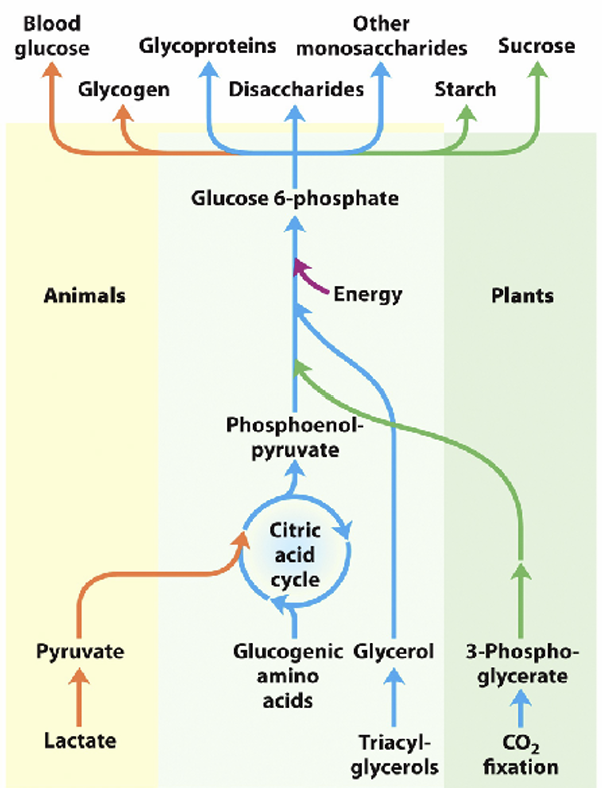
\includegraphics[width=0.5\linewidth]{overview.png}
    \caption{overview of the gluconeogenesis pathway}
    \label{fig:enter-label}
\end{figure}
The body consumes on average around 160g of glucose per day and has storage for 210g. For cells whose sole energy source is glucose this poses a real problem. This is where Gluconeogenesis comes in. In its complete version gluconeogenesis occurs in the \textbf{ liver and kindey cortex.} The main precursors are \textbf{pyruvate, lactate, glycerol and amino acids}. 
\paragraph{total reaction}
$2 Pyruvate + 4 ATP + 2 GTP + 2 NADH + 2 H^{+} + 6 H_2O \rightarrow 
Glucose + 4 ADP + 2 GDP + 6 P_i + 2 NAD^{+}$

\subsection{pathway steps}
\subsubsection{comparison to glycolysis}
\begin{figure}[H]
    \centering
    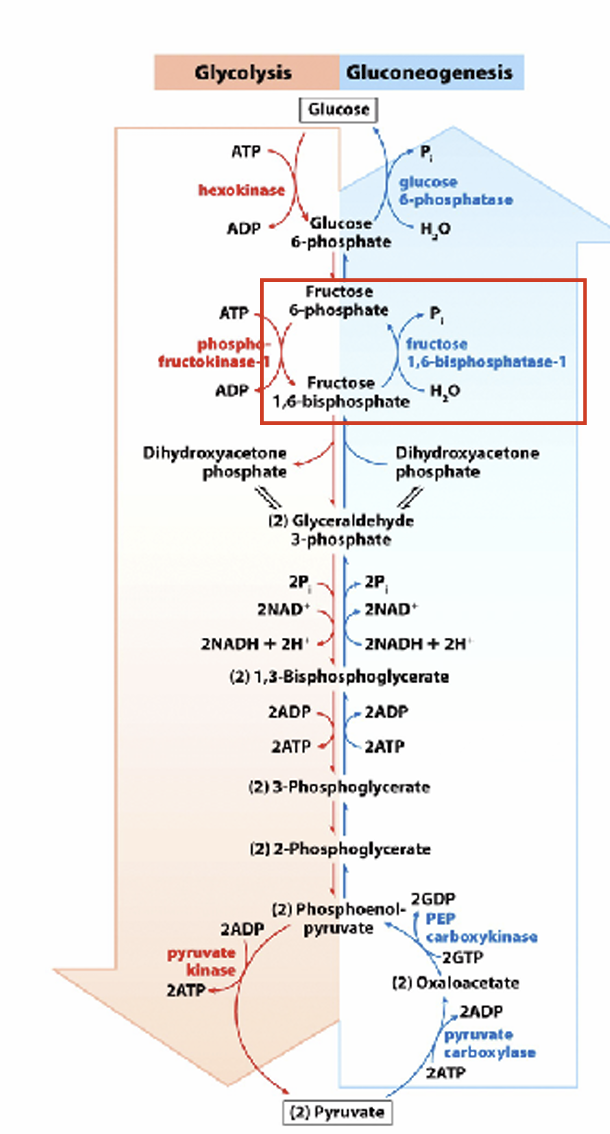
\includegraphics[width=0.5\linewidth]{GlycolysisComparison.png}
    \caption{gluconeogenesis and glycolysis side by side}
    \label{fig:enter-label}
\end{figure}
It differs from glycolysis in the 3 highly exergonic (and thus 'irreversible') reactions:
\begin{itemize}
    \item 1. $glucose + ATP \rightarrow Glucose-6-phophate$
    \item 3. $ fructose-6-phosphate + ATP \rightarrow fructose-1,6-biphosphate$
    \item 10. $ phosphoenolpyruvate + ADP \rightarrow pyruvate + ATP$
\end{itemize}
These reactions have different enzymes compared to glycolysis and are crucial for regulation. All other reactions are identical to glycolysis. 
\subsubsection{step 1 + 2: Pyruvate + ATP $\rightarrow$ PEP}

\begin{figure}[H]
	\centering
	\subfigure[overview of step 1]{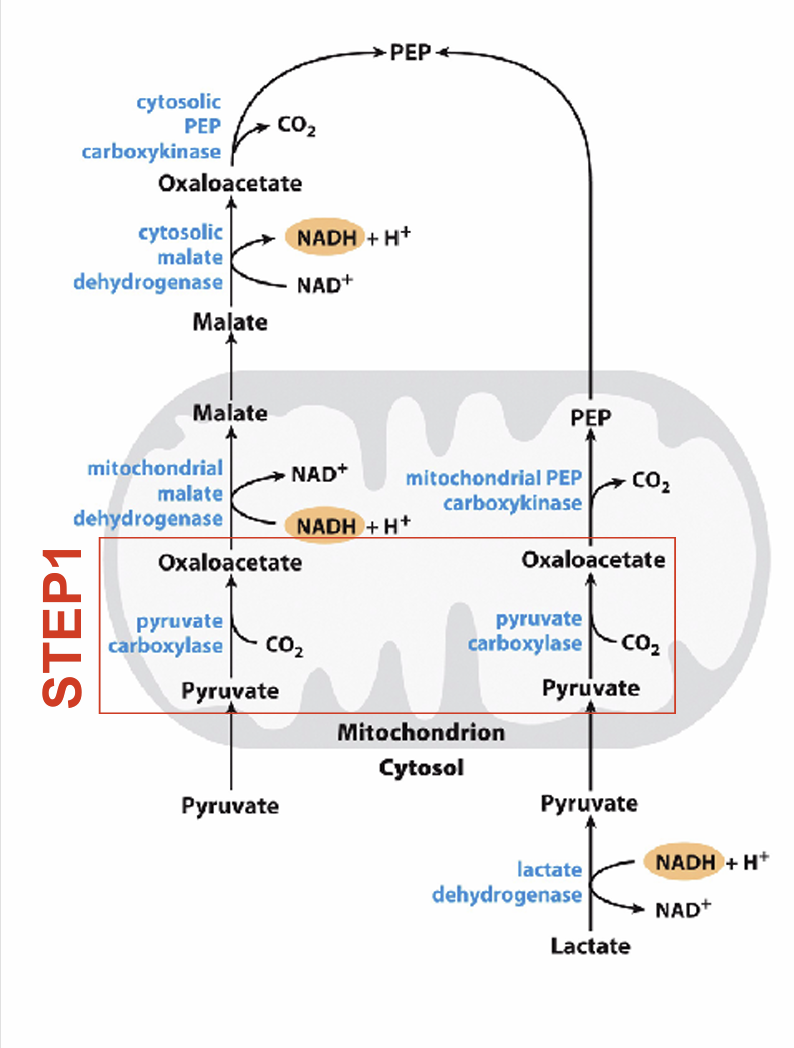
\includegraphics[width = 0.4\textwidth]{step1overview2.png}}
	\subfigure[reaction part 1]{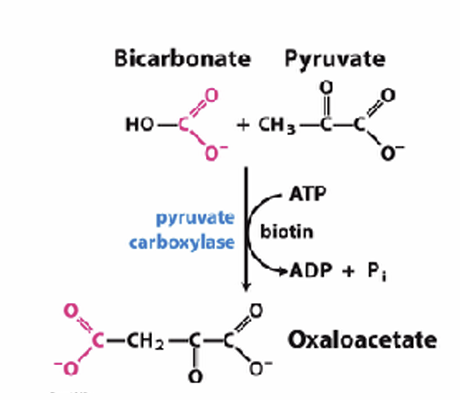
\includegraphics[width = 0.4\textwidth]{step1reaction.png}}

    \subfigure[reaction part 2]{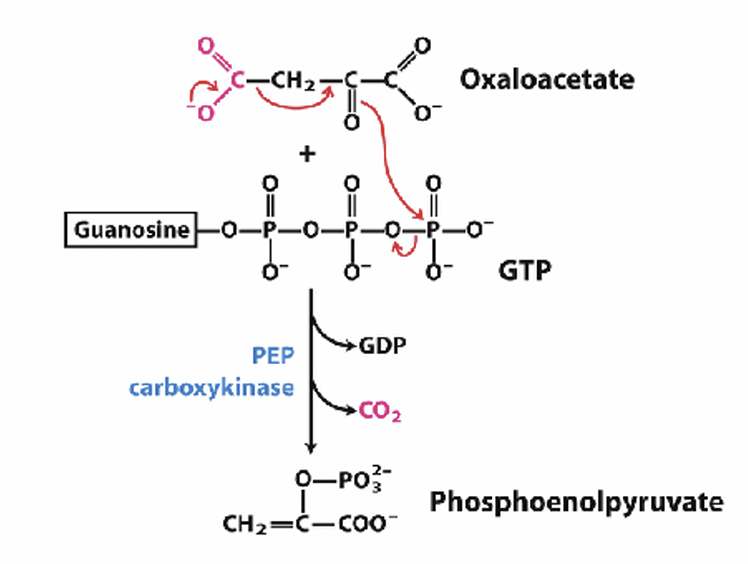
\includegraphics[width = 0.4\textwidth]{step2.png}}
	\caption{step 1 of gluconeogenesis}
\end{figure}


\begin{enumerate}
    \item Pyruvate makes it to the mitochondrial matrix.
    \item In the mitochondria, pyruvate is carboxylated to oxaloacetate by \textbf{\gls{pyruvatecarboxylase}.}
    \item Oxaloacetate is either transformed to PEP by mitochondrial \textbf{\gls{PEPcarboxykinase} }or converted to malate by \textbf{\gls{malatedehydrogenase}.}
    \item Malate (Malate shuttle) and PEP are transported to the cytosol.
    \item Malate is reconverted into oxaloacetate by \textbf{cytosolic \gls{malatedehydrogenase}.}
    \item Oxaloacetate is transformed to PEP by \textbf{cytosolic \gls{PEPcarboxykinase}.}
\end{enumerate}

\begin{RemarkWithTitel}{Malate shuttle}
	    Oxaloacetate can not be exported as such by mitochondria. This is why it is converted to malate and then reconverted to oxaloacetate. This has the effect that \textbf{1 NADH is "transferred" from mitochondria to cytosol}, helping to increase cytosolic NADH.\\
	    \indent When cytosolic NADH is low, and gluconeogenesis requires NADH (e.g., for converting 1,3-BPG to G3P), the malate shuttle is used to generate cytosolic NADH.\\
	    \indent In contrast if lactate is available, lactate to pyruvate (by LDH) actually produces NADH in the cytosol, so the malate shuttle may not be needed — because there's already enough NADH.
\end{RemarkWithTitel}

\paragraph{pyruvate carboxylase mechanism and endergonic - exergonic coupling }
\begin{figure}[H]
    \centering
    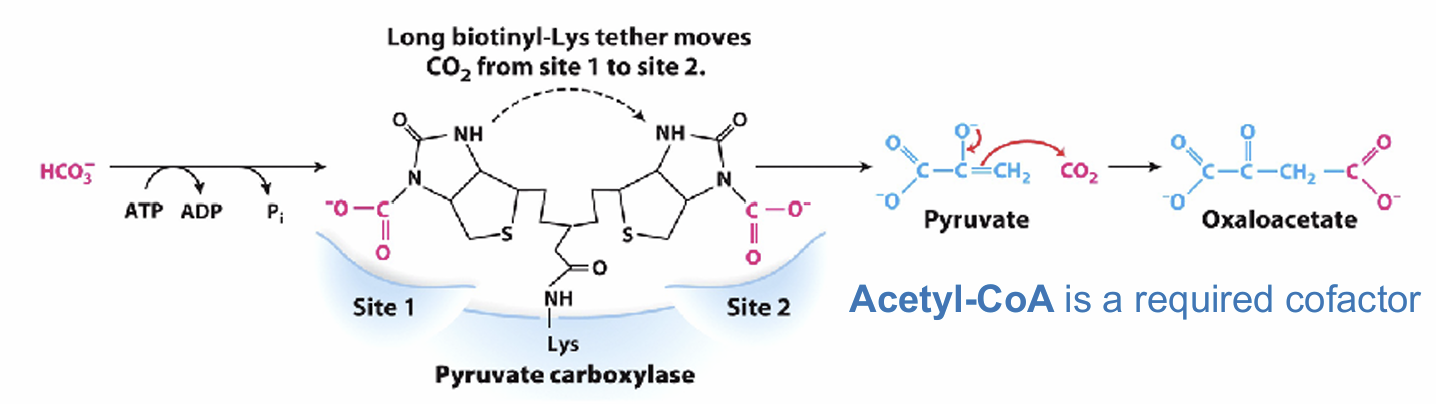
\includegraphics[width=\linewidth]{pyruvateCarboxylase.png}
    \caption{pyruvate carboxylase mechanism}
    \label{fig:enter-label}
\end{figure}
This enzyme is a tetramere, each monomere has a\textbf{ biotin-binding domain} that complexes with CO\textsubscript{2}  and an \textbf{ATP binding domain} The mechanism is as follows:

\begin{enumerate}
    \item \textbf{Phase 1:} ATP activates CO\textsubscript{2}, forming carboxyphosphate.
    \item \textbf{Phase 2:} Phosphorylated CO\textsubscript{2} is attached to the biotin-enzyme with inorganic phosphate (Pi) release.
    \item \textbf{Phase 3:} The CO\textsubscript{2} is transferred to pyruvate to form oxaloacetate.
\end{enumerate}

\textbf{Pyruvate carboxylase requires \gls{acetylcoa} as a cofactor}

\begin{remark}
     The highly endergonic phosporylation that impeded the direct inverse of glycolysis is coupled to the highly exegonic decarboxylation, making this a net exergonic reation.
\end{remark}


\subsubsection{step 8: fructose-1,6-biphophate $\rightarrow$  fructose-6-phosphate}
\begin{figure}[H]
    \centering
    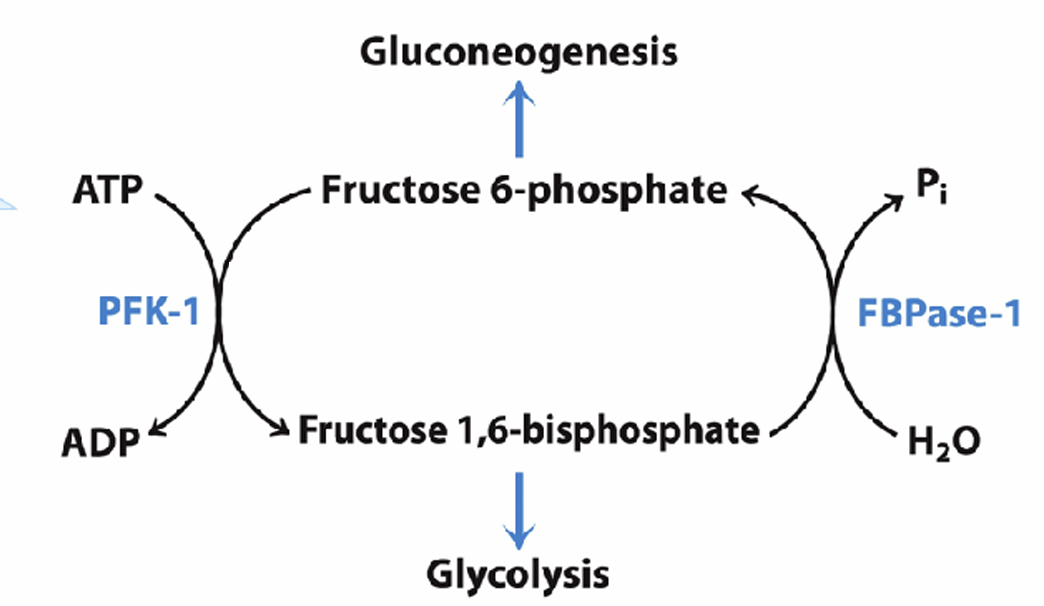
\includegraphics[width=0.5\linewidth]{step8.png}
    \caption{step 8 of gluconeogenesis}
    \label{fig:enter-label}
\end{figure}
Note that step 8 is also not a direct reversal of glycolysis as the FBPase-1 hydrolyses a organic phosphate off instead of transfering it to ADP. \textbf{PFK-1 and FBPase-1 are highly regulated enzymes} See chapter on glucoenogenesis regulation.
\subsubsection{step 10: glucose-6-phosphate $\rightarrow$ glucose}

\begin{figure}[H]
	\centering
    \subfigure[step 10 of gluconeogenesis]{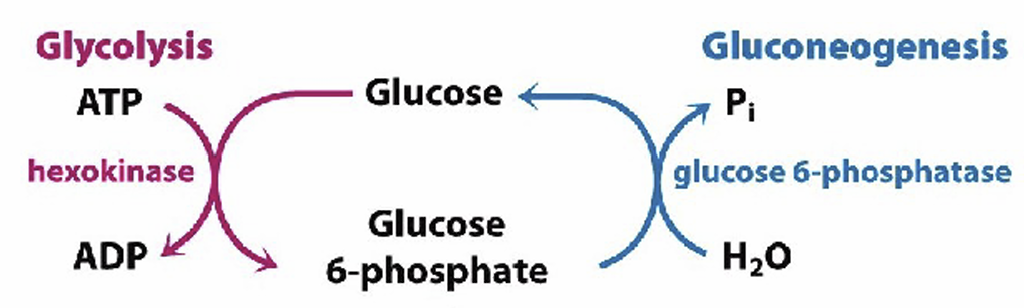
\includegraphics[width = 0.4\textwidth]{step10.png}}
    \subfigure[enzymatic overview]{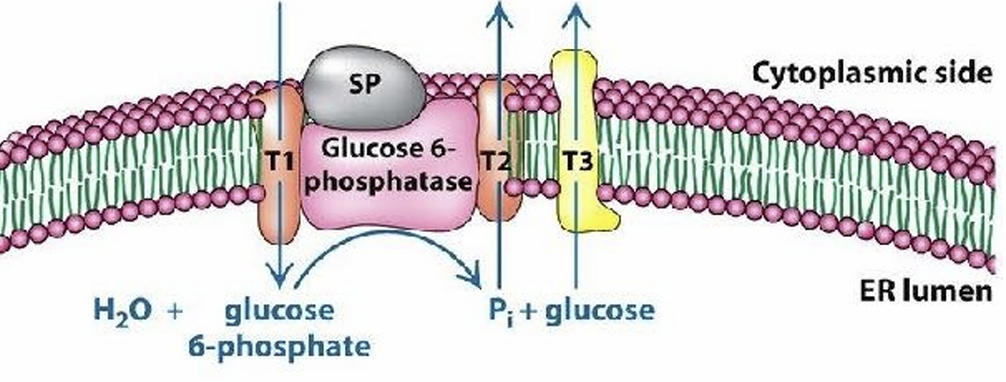
\includegraphics[width = 0.55\textwidth]{step10part2.png}}
	\caption{step 10 of gluconeogenesis}
\end{figure}
This is similar to step 8 however there is an interesting topological consideration:
\begin{enumerate}
    \item \gls{glc6ptransporter} (T1) imports glucose-6-phosphate (Glc(6)P) into the ER lumen.
    \item \gls{glc6ptase} converts Glc(6)P to glucose and inorganic phosphate (Pi).
    \item The reaction is stabilized by the calcium-binding protein \gls{sp} (stabilizing protein).
    \item Pi is transported to the cytosol by the \gls{phosphatetransporter} (T2).
    \item Glucose is transported to the cytosol by the \gls{glucosetransporter} (T3).
\end{enumerate}

\subsection{Regulation}
\begin{remark}
    In general low energy states (low ATP, high ADP and  AMP) favor catabolic pathways such as glycolysis. While high energy states favor anabolic states such as gluconeogenesis. These processes are\textbf{ regulated at cell autonomus} level, i.e each cell does whatever they want. But they are \textbf{also regulated at the organism level}. See chapter on metabolic integration for organism level regulation. 
\end{remark}
\subsubsection{Acetyl-CoA activation}
\begin{figure}[H]
    \centering
    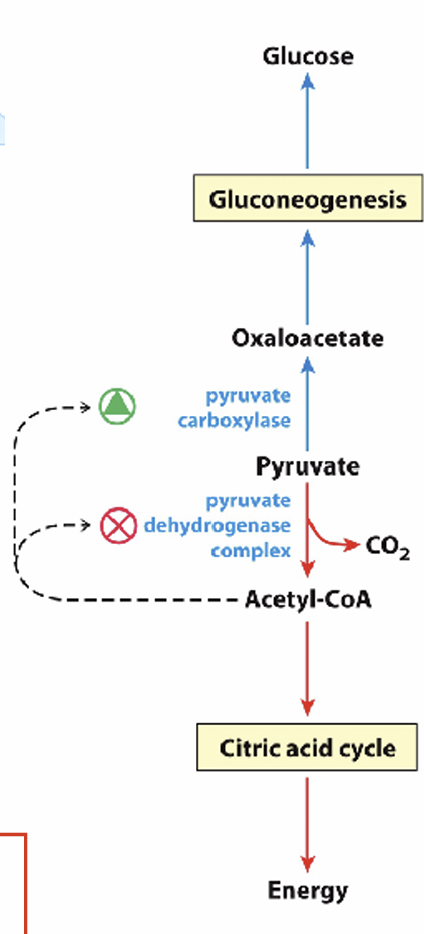
\includegraphics[width=0.3\linewidth]{Acetyl-CoAInhibition.png}
    \caption{Acetyl-CoA inhibition}
    \label{fig:enter-label}
\end{figure}
Acetyl CoA activates \textbf{ \gls{pyruvatecarboxylase}} which is required to form oxaloacetate. This mechanism is useful as \textbf{when Acetyl-CoA accumulates, due to saturation of the TCA cycle it can be fed into gluconeogenesis}

\subsubsection{PFK-1/ FBPase-1 regulation (autonomous level)}
\begin{figure}[H]
	\centering
	
    \subfigure[ATP and it's derivatives effect]{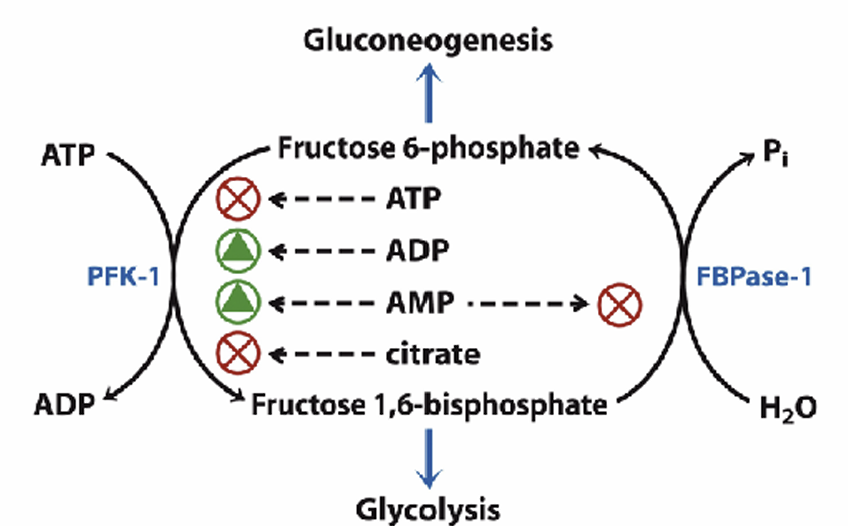
\includegraphics[width = 0.5\textwidth]{PFKreg.png}}


    \subfigure[fructose-2,6-biphosphate effects]{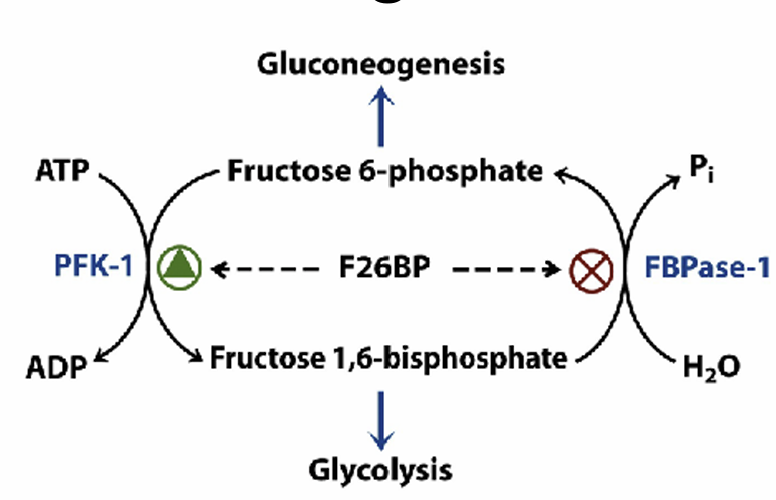
\includegraphics[width = 0.5\textwidth]{regulationPFK1.png}}
	\caption{step 1 of gluconeogenesis}
\end{figure}

\gls{pfk1} is\textbf{ activated by ADP and AMP}, both molecules that are present under low energy conditions. on the otherhad it is \textbf{inhibited by ATP and citrate}, these are present in excess when the cell has a lot of energy. 
\par
\textbf{\gls{fbpase1} is inhibited by AMP}, which is a molecule present at low energy levels.
\par
On top of this it \textbf{PFK-1 is activated by Fructose2,6-biphosphate while FBPase-1 is inactivated} 

\begin{remark}
    \textbf{PFK-1 and PFK-2 are not the same thing.} These are different enzymes with different regulations, same thing for the phsophatases!!
\end{remark}


\subsubsection{PFK-2/ FBPase-2 regulation on organism level (insulin and glucagon)}
This is a bifunctional enzyme that has both a kinase domain (\textbf{\gls{pfk2domain}}) and a phosphatase domain (\textbf{\gls{fbpase2domain}}). This enzyme is responsible for organism level regulation of glycolysis gluconeogenesis.
\begin{figure}[H]
    \centering
    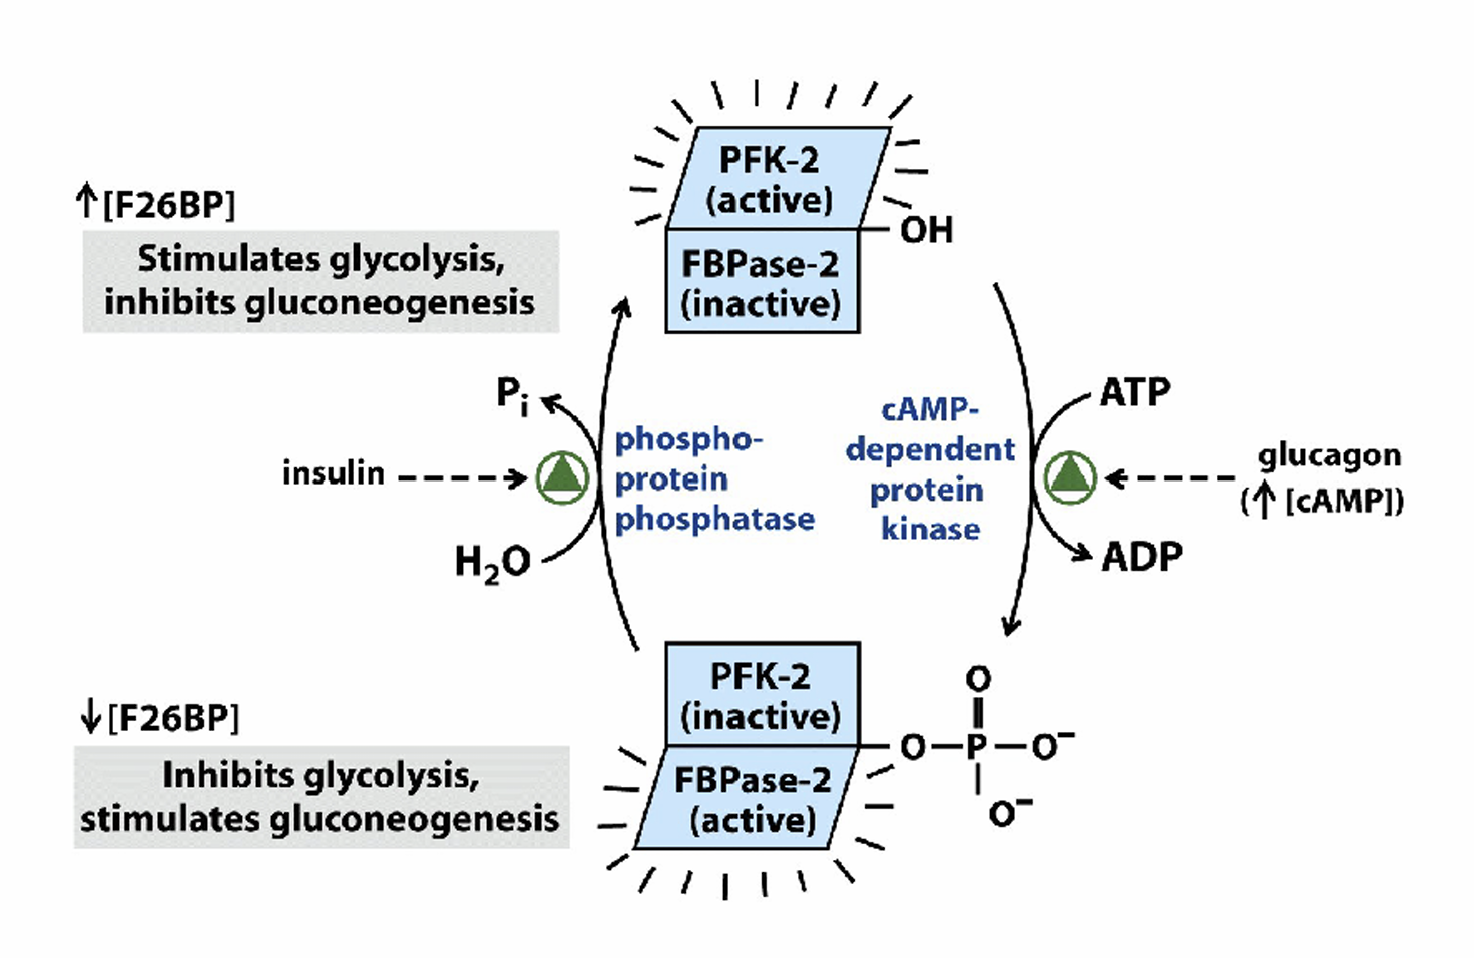
\includegraphics[width=0.5\linewidth]{RegulationInsulin.png}
    \caption{bifunctional enzyme domains integrate insulin and glucagon signals}
    \label{fig:enter-label}
\end{figure}
This enzyme reacts to insulin and glucagon to either increase or decrease the concetration of\textbf{ Fructose-2,6-biphophate (F26BP)}
\begin{itemize}
    \item \textbf{insulin activates PFK-2 domain }that increases F26BP concentrations  this then activates PFK-1 that stimulate glycolysis and inhibit gluconeogenesis.
    \item \textbf{glucagon on the other hand activate FBPase-2 domain} that decreases F26BP concertations that then inturn removes an inhibitor of gluconeogenesis stimulating it more. 
\end{itemize}
\begin{figure}[H]
    \centering
    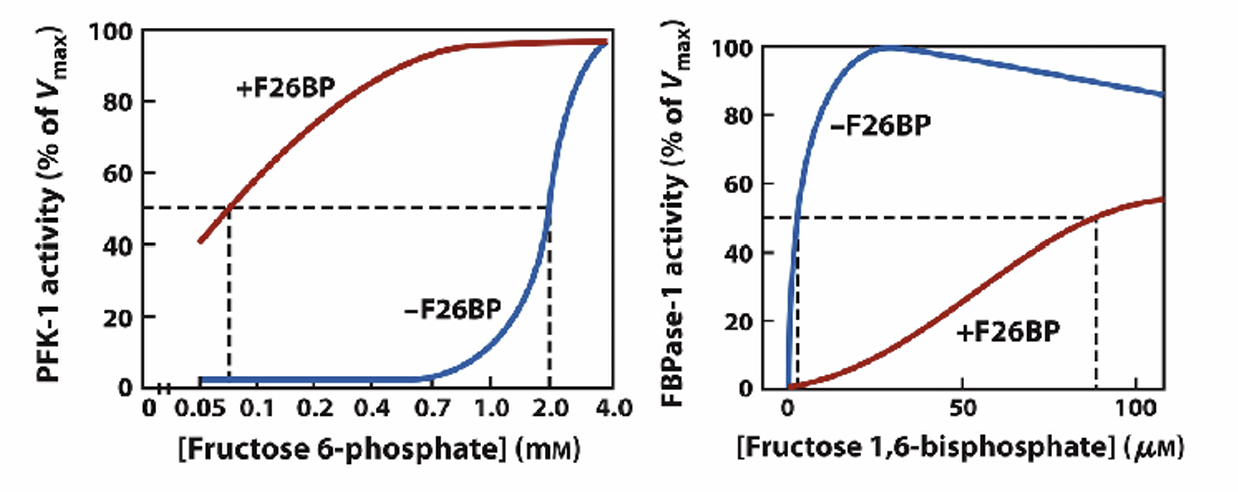
\includegraphics[width=\linewidth]{graph.png}
    \caption{effect of F26BP on glycolysis and gluconeogenesis}
    \label{fig:enter-label}
\end{figure}
This is seen when looking at relative vmax of PFK-1 and FBPase-1. \textbf{PFK-1 is massivly activated by the presence of F26BP} while it has the opposite\textbf{ effect on FBPase-1 acting as an inhibitor}

\section{glycogen metabolism}
\begin{figure}[H]
    \centering
    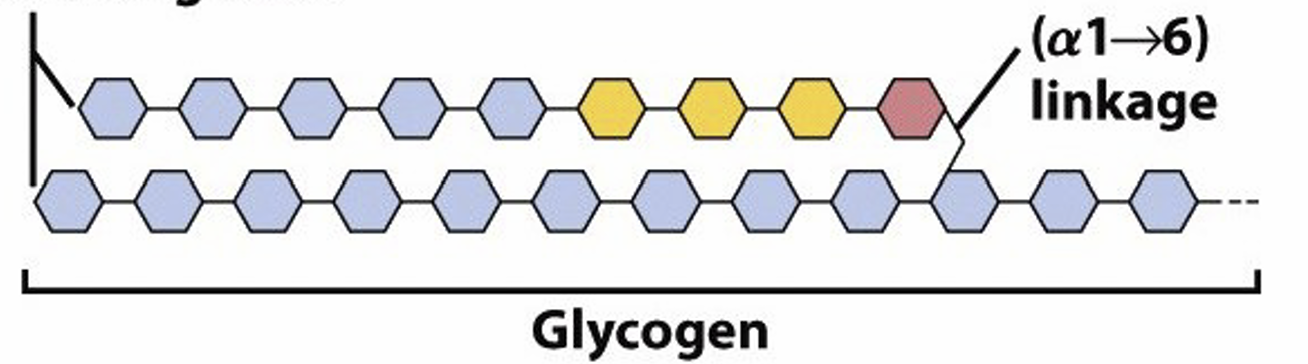
\includegraphics[width=\linewidth]{Glycogen.png}
    \caption{glycogen structure}
    \label{fig:enter-label}
\end{figure}
Glycogen is a storage polymer that is use by liver cells to regulate the blood sugar level. It is a branched polymer consisting of two types of bonds
\begin{enumerate}
    \item $\alpha$(1$\rightarrow$6) bonds: these are the bonds that form the branching points
    \item $\alpha$(1$\rightarrow$4): These bonds are the ones that extend the polymer 
\end{enumerate}
\subsection{glycogenesis}
\subsubsection{step 1: Glucose activation}
\begin{figure}[H]
	\centering
	\subfigure[reaction]{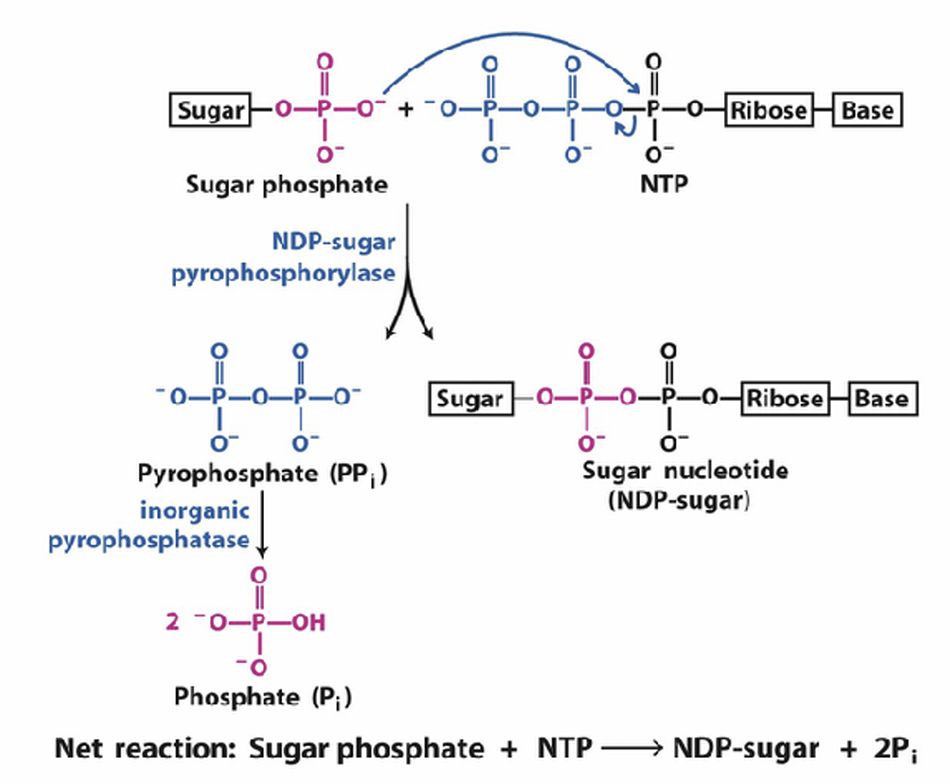
\includegraphics[width = 0.5\textwidth]{UDP1.png}}
	\subfigure[UDP structure]{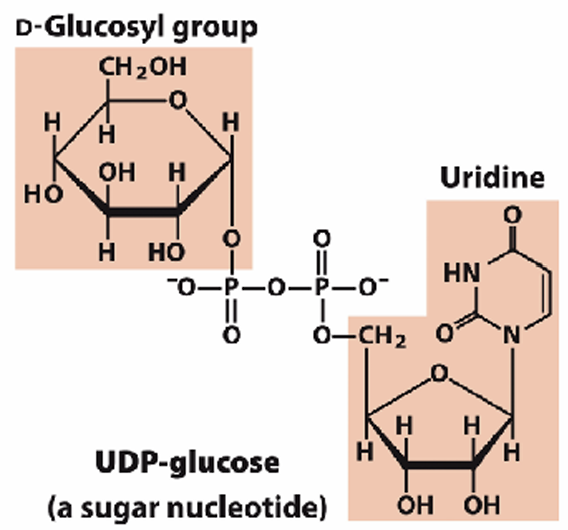
\includegraphics[width = 0.4\textwidth]{UDPstructure.png}}
	\caption{glucose activation}
\end{figure}
\textbf{\gls{udp-glucose-pyrophosphorylase}} to transform a 
\textbf{glucose 1-phosphate} into a uridine diphosphate glucose (\textbf{UDP-glucose)}. This reaction produces a 
pyrophosphate, which then is hydrolyzed by water to form two orthophosphate 
molecules.\textbf{ This second step drives the reaction forward}

\begin{remark}
    note that glucose-1-phosphate is not the glucose that arrives from glycolsis (that would be glucose-6-phosphate) It thus needs to be isomerized by \textbf{\gls{phosphoglucomutase}}
\end{remark}
\subsubsection{step2: creating the primer}
\begin{figure}[H]
    \centering
    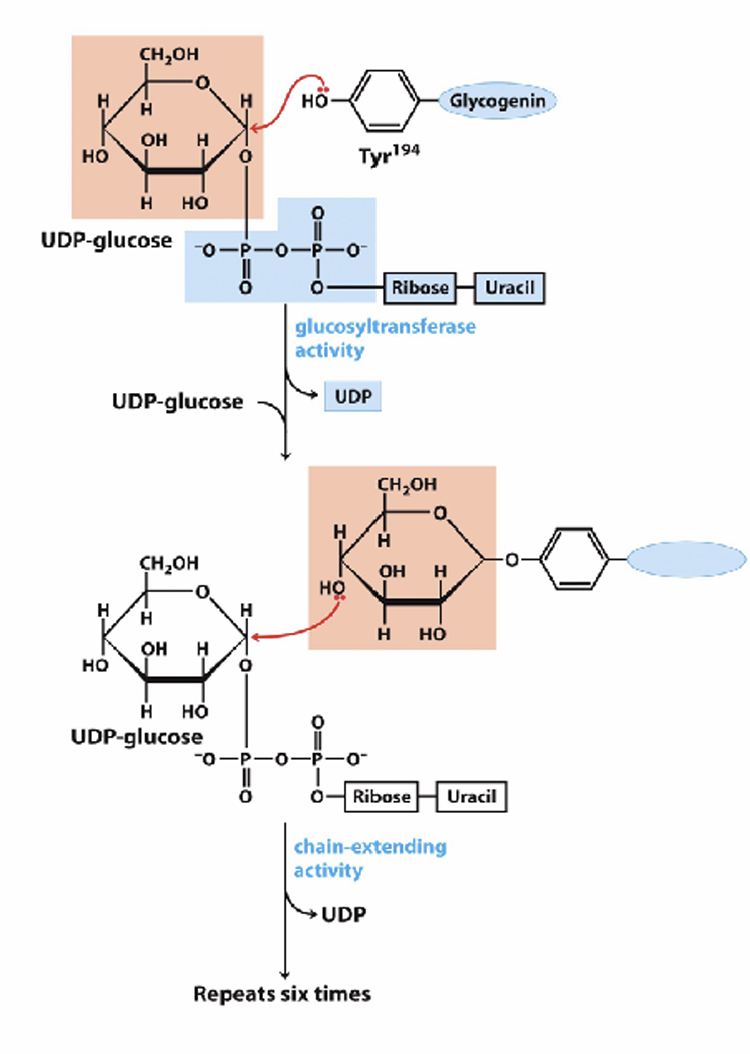
\includegraphics[width=0.5\linewidth]{primer.png}
    \caption{glycogenin autocatalyzes the addition of UDP onto itself}
    \label{fig:enter-label}
\end{figure}
\begin{enumerate}
    \item \textbf{Transfer of a glucose residue:} A glucose residue from UDP-glucose is transferred to a tyrosine residue of \textbf{\gls{glycogenin}}. This reaction is catalyzed by glycogenin itself.
    \item \textbf{Chain extension:} Glycogenin catalyzes the sequential addition of seven more glucose units, forming a short primer of\textbf{ $\alpha$(1$\rightarrow$4)-linked glucose residues.}
\end{enumerate}

This leads to the formation of the \textbf{8-monomer-primer} that will subsequently be elongated.
\subsubsection{step 3: elongation}
\begin{figure}[H]
    \centering
    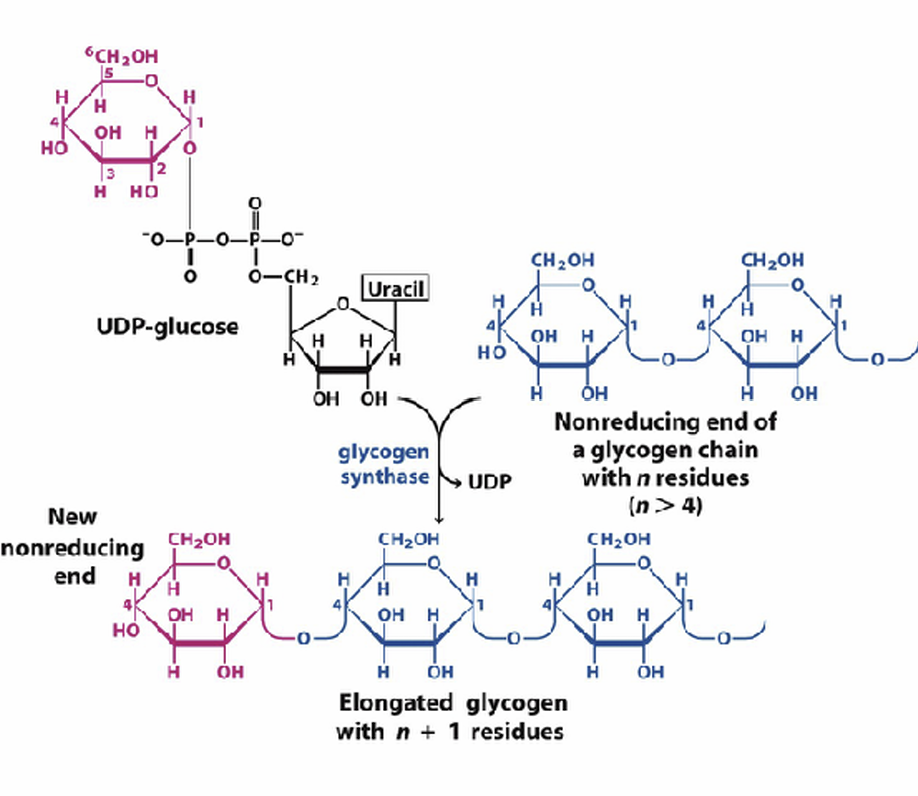
\includegraphics[width=0.5\linewidth]{elongation.png}
    \caption{elongation of glycogen}
    \label{fig:enter-label}
\end{figure}
\textbf{\gls{glycogen-synthase}} catalyzes the addition of further UDP-glucose molecules by\textbf{ catalyzing the formation of  $\alpha$(1$\rightarrow$4) glycosidic bonds }

\subsubsection{branching}
\begin{figure}[H]
    \centering
    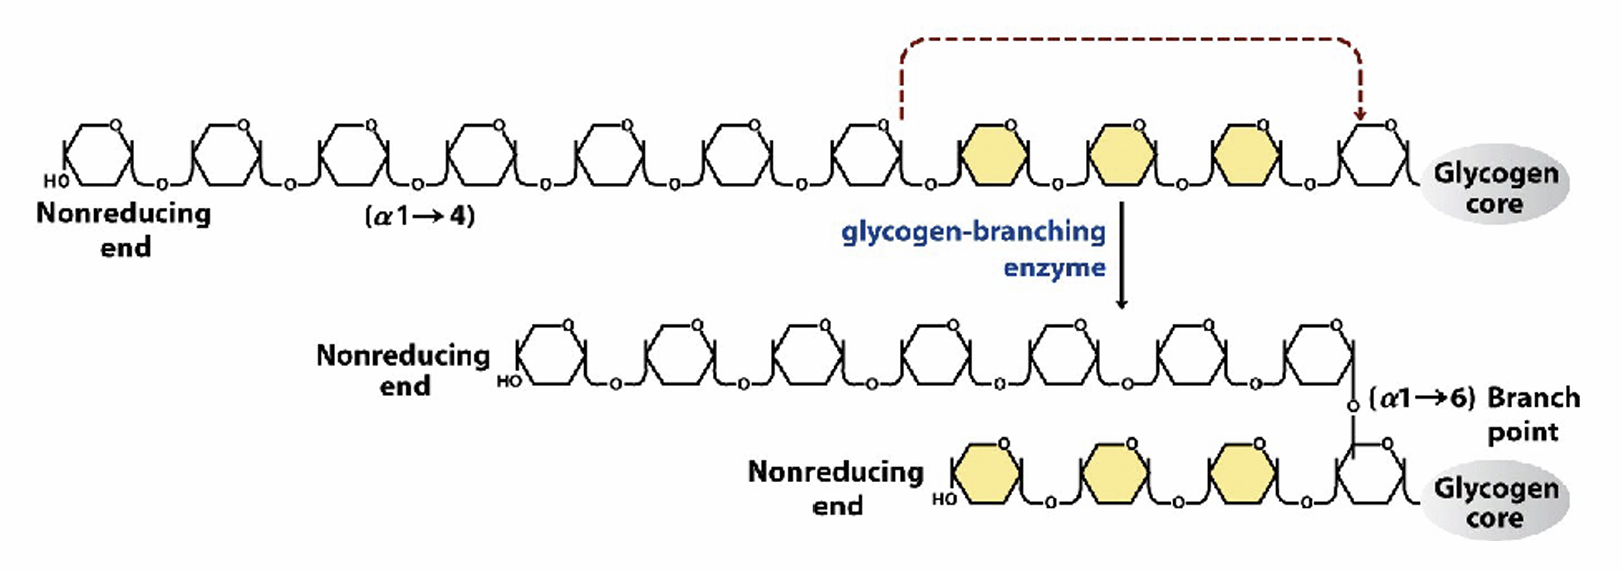
\includegraphics[width=\linewidth]{branching.png}
    \caption{branching}
    \label{fig:enter-label}
\end{figure}

Branching is a way to \textbf{increase the solubility} of glycogen as well as increase the number of non-reducing ends which will allow for \textbf{faster breakdown} This is catalyzed by the \textbf{formation of  $\alpha$(1$\rightarrow$6) glycosidic bonds by \gls{glycogen-branching-enzyme}}
\par
\textbf{Glycogen-branching enzyme catalyzes} the transfer of a terminal fragment (6 or 7 residues long) from the nonreducing end of a branch (at least 11 residues long) to the C-6 hydroxyl group of a glucose residue on the same chain or another chain creating a branch with an $\alpha$(1$\rightarrow$6) linkage

\subsection{glycogen breakdown}
\begin{figure}[H]
    \centering
    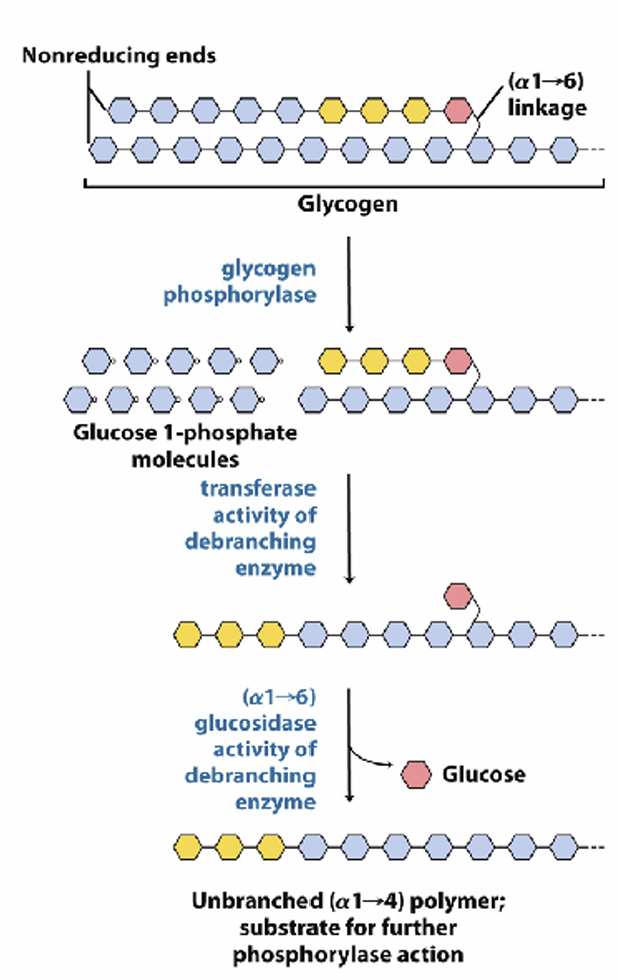
\includegraphics[width=0.4\linewidth]{breakdownGlycogen.png}
    \caption{glycogen breakdown}
    \label{fig:enter-label}
\end{figure}


\begin{enumerate}
    \item \textbf{Phosphorolysis:} The first step is catalyzed by glycogen phosphorylase, which uses orthophosphate (\( \text{P}_{\text{i}} \)) to cleave the glycosidic bond between a terminal glucose unit (with a free hydroxyl group) and the rest of the glycogen molecule. This reaction produces glucose-1-phosphate and a glycogen molecule shortened by one glucose residue.

    \item \textbf{Branch point limitation:} Glycogen phosphorylase cannot cleave the \(\alpha(1\rightarrow6)\) glycosidic bonds at the branching points. It stops cleaving when it is four glucose residues away from such a branch.

    \item \textbf{Debranching enzymes:} A transferase enzyme shifts a block of three glucose residues from the branch to a nearby linear chain. Then, an \(\alpha(1\rightarrow6)\) glucosidase hydrolyzes the remaining single glucose residue at the branch point, releasing a free glucose.

    \item \textbf{Conversion to glucose-6-phosphate:} Finally, phosphoglucomutase converts the glucose-1-phosphate produced in the first step into glucose-6-phosphate, which can then enter glycolysis or other metabolic pathways.
\end{enumerate}
\subsection{glycogen regulation}
\begin{figure}[H]
    \centering
    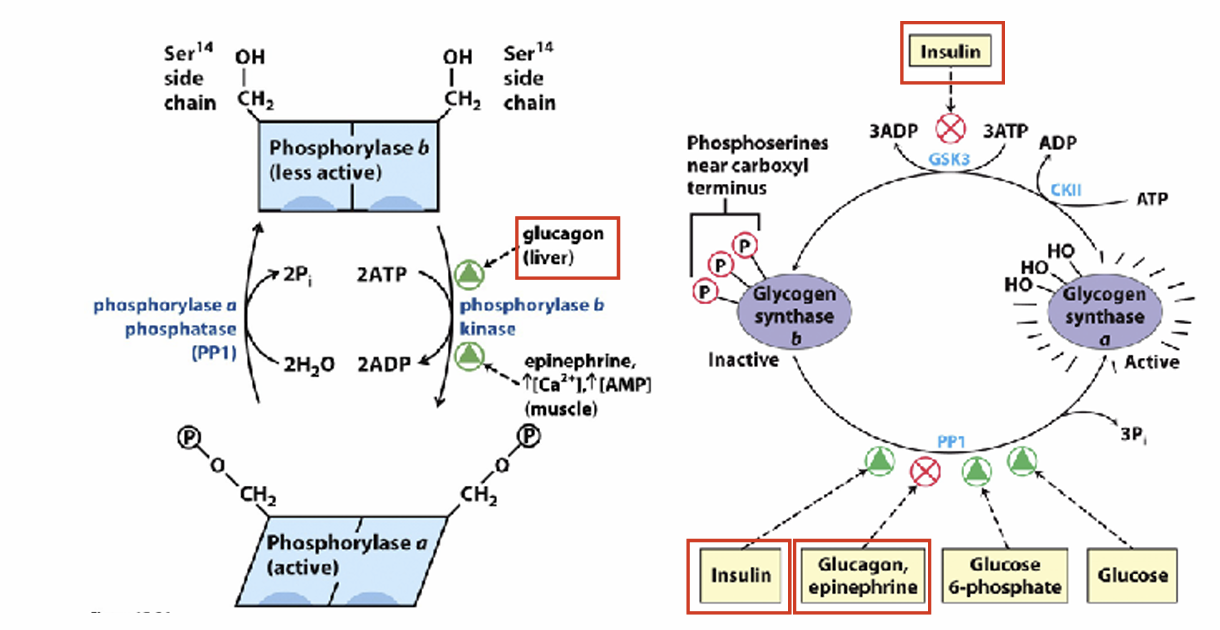
\includegraphics[width=\linewidth]{glycogenregulation.png}
    \caption{glycogen Regulation}
    \label{fig:enter-label}
\end{figure}
Glycogen metabolism consists of two processes - glycogen synthesis and glycogen degradation. These two processes however do not take place the same moment in time. In fact, our body has a mechanism in place that regulates them in a reciprocal fashion - 
\textbf{when one process is on, the other process is off.} \textbf{Glycogen phosphorylase and glycogen synthase are reciprocally regulated}






\end{document}